\section{Stochastic vehicle dynamic framework}
\label{sec:svdf}

\subsection{Vehicle model}
\label{sec:vehicle_model}
The vehicle model employed in this study is a Single Track model featuring nonlinear axle characteristics. A schematic representation of the Single Track model is shown in Fig.~\ref{fig:vehicle_model}. The lateral forces $Y_1$ and $Y_2$ are computed using a Pacejka's Magic Formula, which depends on the total vertical load acting on the axle and the axle's apparent slip angle.
The longitudinal forces $X_1$ and $X_2$ are provided as inputs to the system. Specifically, the first two components of the input vector $\bu$ correspond to acceleration and braking forces, while the third component represents the steering angle of the front wheels. This input formulation facilitates the distribution of braking forces between the front and rear axles, while assigning acceleration exclusively to the rear axle, consistent with the rear-wheel-drive configuration of the modeled vehicle.

By treating the longitudinal forces as inputs, the longitudinal dynamics can be explicitly solved, allowing the computation of vertical load transfers prior to their use in the expression of the lateral forces. Consequently, the time derivative of the state becomes an explicit function of the state vector $\bx$ and the input vector $\bu$, as follows:
\begin{equation}
	\dbx(t) = f(\bx(t), \bu(t))
\end{equation}

The state vector $\bx$ has six components and includes the three kinematic quantities $u$, $v$, and $r$, along with the position $\left(x_G, y_G\right)$ and orientation $\psi$ of the barycentrical reference frame. As illustrated in Fig.~\ref{fig:vehicle_model} $u$ and $v$ represent the longitudinal and lateral velocity of the CoM w.r.t its reference frame, while $r$ represents vehicle's yaw rate.

\begin{figure}
	\centering
	\begin{tikzpicture}[scale=2, x = {(0,1cm)}, y = {(-1cm,0)},
	force/.style={->, thick, red!60!black, >={Latex[length=10pt, width=4pt]}},
	vec/.style={->, thick, mgreen, >={Latex[length=10pt, width=4pt]}},
	aux/.style={thin},
	frame/.style={->,thin,>={Latex}},
	every node/.style={font=\small, text=black}
	]
	\definecolor{mgreen}{RGB}{0,100,0}
	\begin{scope}[rotate = 25,shift = {(-.3,-2)}]
		% Coordinates
		\coordinate (rear) at (0,0);
		\coordinate (G) at (1.2,0);
		\coordinate (front) at (2.8,0);
		
		% Main body line
		\draw[blue!50!black, thick] (rear) -- (front);
		
		% Rear wheel
		\draw[fill=black!60!white, draw=black, rounded corners=2pt]
		($(rear)+(-.2,.1)$) rectangle ($(rear)+(+.2,-.1)$);
		
		% Front wheel (rotated around its center)
		\begin{scope}[shift={(front)}, rotate=25]
			\draw[fill=black!60!white, draw=black, rounded corners=2pt]
			(-0.2,.1) rectangle (0.2,-.1);
		\end{scope}
		
		% Local axes at rear
		\draw[force] (rear) -- ++(.5,0) node[above,right] {$X_2$};
		\draw[force] (rear) -- ++(0,1.3) node[above] {$Y_2$};
		
		% Local axes at front
		\draw[force] (front) -- ++(-.3,0) node[right] {$X_1$};
		\draw[force] (front) -- ++(0,1.5) node[above] {$Y_1$};
		
		% Velocity vectors at G
		\draw[vec] (G) -- ++(.6,0) node[left, shift={(-.2,-.1)}] {$u\,\mathbf{i}$};
		\draw[vec] (G) -- ++(0,.3) node[above] {$v\,\mathbf{j}$};
		
		% Angular velocity
		\begin{scope}[rotate = -115]
			\draw[vec] 
			(-.1,.8) arc[start angle=0, end angle=50, radius=1]
			node[midway, right=2pt] {$r\,\mathbf{k}$};
		\end{scope}
		
		% G point
		\fill (G) circle (1pt) node[right] {$G$};
		
		% Body frame
		\draw[frame] (G) --++ (1,0) node[right] {$x_b$};
		\draw[frame] (G) --++ (0,1) node[above] {$y_b$};
		
		% Distances
		%			\draw[<->,>={Latex}] (3,-1) -- node[left] {$a_1$} (1.5,-1);
		%			\draw[<->,>={Latex}] (1.5,-1) -- node[left] {$a_2$} (0,-1);
		
		% Steering angle (auxiliary vertical line)
		\draw[aux] (front) -- ++(.4,0);
		\draw[aux] (front) -- ++({0.4*cos(25)}, {0.4*sin(25)});
		
		% Steering angle arc
		\draw[->,thin,>={Latex}] ([shift={(0.35,0)}]front) arc[start angle=0, end angle=25, radius=0.35];
		\node[left,shift={(.15,0)}] at ([shift={(0.35,0)}]front) {$\delta$};
		
		% Psi angle aux
		\draw[aux] (G) -- ++({0.4*cos(25)}, {-0.4*sin(25)});
		
		% Psi angle
		\draw[->,thin,>={Latex}] ([shift={({0.35*cos(25)},{-.35*sin(25)})}]G) arc[start angle=-25, end angle=0, radius=0.35];
		\node[left,shift={(.2,-.05)}] at ([shift={({0.35*cos(25)},{-.35*sin(25)})}]G) {$\psi$};
		
	\end{scope}
	\coordinate (ground) at (0,0);
	\draw[frame] (ground) --++ (1,0) node[right] {$x$};
	\draw[frame] (ground) --++ (0,1) node[above] {$y$};
	\draw[->,thick,>=Latex] (ground) --++ (G);
	%		\draw[->,thick,>=Latex] (ground) --++ (G) node[midway, shift={(0,-.3)}] {$\boldsymbol{p}$};
	
\end{tikzpicture}
	%\caption{Single Track model. The ground force acting on each axle is decomposed into longitudinal and lateral components, indicated by red arrows. The longitudinal components are part of the input vector $\bu$, encompassing both acceleration and braking forces, while the lateral components are computed using Pacejka's Magic Formula based on the vertical load and slip angle at each axle. The figure also depicts the fixed reference frame and the body reference frame, with the origin located at the vehicle's center of mass (CoM). The state variables $u$ and $v$ represent the longitudinal and lateral velocities of the CoM w.r.t. the body frame, while $r$ denotes the yaw rate. The angle $\psi$ is used to describe the orientation of the body frame w.r.t. the fixed frame.}
	\caption{Single Track model.}
	\label{fig:vehicle_model}
\end{figure}

\subsection{Stochastic vehicle dynamics}
\label{sec:stochastic_vehicle_dynamics}

We model the \emph{perturbed vehicle dynamics} as the following nonlinear continuous-time random dynamical system
\begin{align}
\dbx(t) = f(\bx(t), \bu(t)) + \bw(t),
\end{align}
where $\bu(t)$ are the deterministic control inputs, $\bw(t)$ is additive Gaussian white noise with zero mean and known covariance $\bQ(t)$, i.e. $\bw(t) \sim \calN(\bzero, \bQ(t))$, and $\bx(t)$ is the state vector.
Assuming a \emph{first-order} approximation for the disturbance propagation rule, $\bx(t)$ results in a Gaussian distribution with mean $\bmu(t)$ and covariance $\bP(t)$, so that $\bx(t)~\sim~\calN(\bmu(t), \bP(t))$.

Due to the symmetry of the probability density function (pdf) with respect to $\bmu(t)$, it is possible to represent the time evolution of the pdf as: i) the deterministic evolution of the mean $\bmu(t)$
\begin{align}\label{eq:meandynamics}
\dbmu(t) = f(\bmu(t), \bu(t)),
\end{align}
and ii) the time evolution of the state covariance matrix $\bP(t)$ along $\bmu(t)$, which can be expressed by the \emph{Lyapunov matrix differential equation}
\begin{align}\label{eq:dP}
\dbP(t) = \bA(t) \bP(t) + \bP(t) \bA^T(t) + \bQ(t),\quad \bP(0) = \bP_0 = \bP_0^T.
\end{align}
In~\eqref{eq:dP}, $\bP_0$ is the \emph{initial} state covariance and $\bA(t)$ is the usual shorthand notation for the Jacobian along the mean trajectory $\bmu(t)$, that is $\bA(t)=\frac{\pd f(\bmu, \bu)}{\pd \bmu}$.
%\bJ(\bmu(t),\bu(t))$, where $\bJ(\bx, \bu) = \frac{\pd f(\bx, \bu)}{\pd \bx}$.

As can be readily verified by differentiation~\cite{Gajic:LyapunovMatrixEquation:2010}, the analytical solution of~\eqref{eq:dP} has the form
\begin{align}\label{eq:P_STM}
\bP(t) = \bPhi(t,t_0) \bP_0 \bPhi(t,t_0)+\int_{t_0}^{t} \bPhi(t,\tau) \bQ(\tau) \bPhi^T(t,\tau) \dd \tau \quad \bP(0)=\bP_0,
\end{align}
where $\bPhi(t,t_0)$ is the \emph{state transition matrix}. This matrix encodes the evolution from $t_0$ to $t$ of a perturbation w.r.t. to the mean trajectory $\bmu(t)$. In symbols, $\barbx(t) = \bPhi(t,t_0) \barbx(t_0)$, with $\barbx(\cdot) =\bx(\cdot) - \bmu(\cdot) $. In turn, the evolution of $\bPhi(t,t_k)$ from a generic $t_k$ to $t$ is driven by the following differential equation
\begin{align}\label{eq:STM}
\dbPhi(t,t_k) = \bA(t)\bPhi(t,t_k), \quad \bPhi(t_k, t_k) = \bI.
\end{align}
In geometric and orbital mechanics, see e.g.~\cite{Maruskin:DynamicalSystemsGeometric:2018} or~\cite{Tapley:StatisticalOrbitDetermination:2004}, the usual choice for statistical trajectory determination is to employ~\eqref{eq:meandynamics} along with~\eqref{eq:P_STM} and~\eqref{eq:STM}. In our case, since we use collocation integrators for stochastic trajectory planning, we follow a more direct approach -- motivated by~\cite{Gillis:PracticalMethodsApproximate:2015} -- by directly employing~\eqref{eq:meandynamics} and~\eqref{eq:dP}.

Accordingly, the continuous-time stochastic trajectory planning can be framed as the following nonlinear optimal control problem
\begin{subequations}\label{eq:OCP}
\begin{align}
	\underset{\bmu(t), \bu(t), \bP(t)}{\text{minimize}} \quad & J(\bmu(t), \bu(t), \bP(t)) \label{eq:OCPcost} \\
	\text{s.t.} \quad \dbmu(t)           &= f(\bmu(t), \bu(t)) \label{eq:OCPdyn} \\
	\phantom{\text{s.t.} \quad} \bmu(0)  &= \bmu_0 \label{eq:OCPdynIC} \\
	\phantom{\text{s.t.} \quad} \dbP(t) &= \bA(t) \bP(t) + \bP(t) \bA^T(t) + \bQ(t) \label{eq:OCPdP} \\
	\phantom{\text{s.t.} \quad} \bP(0)  &= \bP_0 \succeq 0 \label{eq:OCPdPIC} \\ %& \phantom{\text{s.t.} \qquad} 0       \geq h_i(\bmu(t), \bu(t))
	%+ \overbrace{\gamma \bigg[\underbrace{\na^T_{\bx} h_i \bP(t) \na_{\bx} h_i}_{\text{variance of $h_i(\bx)$}}\bigg]^{\frac{1}{2}}}^{\text{safety margin}},
	\phantom{\text{s.t.} \qquad} 0&       \geq h_i(\bmu(t), \bu(t))
	+ \be_i(\bmu(t), \bu(t), \bP(t)),
	\quad i \in \calI \label{eq:OCPconstraints}
\end{align}
\end{subequations}
The cost function $J$ in~\eqref{eq:OCPcost} depends on the mean $\bmu(t)$, the controls $\bu(t)$ and the state covariance $\bP(t)$. The mean dynamics is expressed by~\eqref{eq:OCPdyn} with~\eqref{eq:OCPdynIC}, and the covariance dynamics is expressed by~\eqref{eq:OCPdP} with~\eqref{eq:OCPdPIC}. In eq.~\eqref{eq:OCPconstraints} the \emph{backoff terms} $\be_i$ account for the disturbances and serve the purpose of obtaining deterministic safety margins directly on $\bmu(t)$. $\calI$ is the set of indices defining the inequality constraints. The backoff terms stem for a linearization around the mean of the original \emph{chance constraint} on $\bx(t)$ expressed by $\Prob \{h_i(\bx) \leq 0\}\geq p$, where $p$ is the confidence level of constraint satisfaction. Explicitly, the backoff terms are given by
$\be_i = \gamma \sig_i$. The coefficient $\gamma = \Phi^{-1}(p)$ is the quantile function, where $\Phi(z)=\Prob \{Z\leq z\}$ is the cumulative distribution function (cdf) of a standard normal distribution $Z \sim \calN(0,1)$, and acts as a \emph{tuning knob}: the greater the confidence level $p$ required, the higher the gain $\ga$\footnote{For example, with $p=0.84$ $\ga = 1.0$, with $p=0.97$ $\ga = 2.0$, with $p=0.99$ $\ga = 3.0$}. The term $\sig_i = \big[\na^T_{\bx} h_i(\bmu) \bP(t) \na_{\bx} h_i(\bmu)\big]^{\frac{1}{2}}$ represents the standard deviation of the constraint $h_i(\bx)$ linearized around the mean, i.e. of random variable $h_i(\bmu)+\na^T_{\bx} h_i(\bmu) (\bx - \bmu)$, and follows immediately from the propagation rule of covariance.

\subsection{Discretization via direct collocation}
\label{sec:discretization}
The nonlinear optimal control problem~\eqref{eq:OCP} can be discretized by applying a suitable collocation integrator obtaining the following nonlinear program (NLP)
\begin{subequations}\label{eq:DOCP}
\begin{alignat}{3}
\underset{\bmu_k,\bxi_k, \bu_k, \bP_k,\bz_k}{\text{minimize}} \,
& & & J_k(\bmu_k,\bxi_k, \bu_k) & & \label{eq:DOCPcost} \\
\hspace*{-2.0 cm}\text{s.t.} \quad
& \bzero      & = & \; \bPsimu_k(\bmu_{k-1},\bmu_k,\bxi_k, \bu_k,\bz_k),
& \quad & k = 1,\ldots, N \label{eq:DOCPdyn} \\
& \bmu_0      & = & \; \bar{\bmu}_0
& & \label{eq:DOCPdynIC} \\
& \bzero      & = & \; \bPsiP_k(\bmu_k,\bxi_k, \bu_k, \bP_{k-1},\bP_k,\bSi_k,\bz_k),
& \quad & k = 1,\ldots, N \label{eq:DOCPdP} \\
& \bP_0       & = & \; \bar{\bP}_0 \succeq 0
& & \label{eq:DOCPdPIC} \\
& \bzero      & = & \; \bOm_k(\bmu_k,\bxi_k, \bu_k,\bz_k),
& \quad & k = 0,\ldots, N \label{eq:DOCPpath} \\
& 0           & \geq & \; h_i(\bmu_k, \bu_k, \bz_k) + \be_i(\bmu_k, \bu_k, \bP_k, \bz_k),
& \quad & k = 1,\ldots, N;\; i \in \calI \label{eq:DOCPconstraints}
\end{alignat}
\end{subequations}
To perform the discretization, the track centerline is parameterized using a curvilinear parameter $\alpha \in [0,1]$, and uniformly sampled at $N+1$ points $\alpha_0, \ldots, \alpha_N$.
Accordingly, $\bmu_k$ denotes the mean state at grid node $\alpha_k$, while the controls $\bu_k$ and the algebraic variables $\bz_k$ are assumed to be piecewise constant over each interval $[\al_k, \al_{k+1}]$.
The $\bz_k$'s are introduced as direct handles for physically meaningful quantities such contact forces. Similarly, $\bP_k$ represents the covariance matrix at the $k$-th node.
Following the direct collocation approach, both the mean and covariance state trajectories are approximated, in the $k$-th interval, with polynomials $\pi_k(\tau)$, defined on the unit interval $\tau\in[0,1]$, and then scaled to match the width $\nu_k$ of the corresponding time step. On the unit interval, we select $d$ collocation points $\tau_1, \ldots, \tau_d$, associated with as many collocation states. Accordingly, we define $\bxi_k$ and $\bSi_k$ as the mean states and covariance matrices at the $d$ collocation points within each interval $[\al_k, \al_{k+1}]$, respectively. Therefore, $\bxi_k =
(\bxi_{k,1}, \ldots, \bxi_{k,d})$, and similarly $\bSi_k=(\bSi_{k,1}, \ldots, \bSi_{k,d})$. Equations~\eqref{eq:DOCPdyn} and~\eqref{eq:DOCPdP} represent the collocation and continuity equations for mean and covariance, respectively, with initial conditions represented by~\eqref{eq:DOCPdynIC} and~\eqref{eq:DOCPdPIC}. Eqs.~\eqref{eq:DOCPpath} are path equality constraints and~\eqref{eq:DOCPconstraints} are the robustified inequality constraints.

In certain cases~\cite{Gillis:PracticalMethodsApproximate:2015}, positive-definiteness-preserving Lyapunov discretization schemes are used in~\eqref{eq:DOCPdP}. However, for sufficiently fine discretization, we found that integrating only the lower triangular part of $\bP(t)$ in~\eqref{eq:OCPdPIC}  (and reconstructing its strictly upper part accordingly), ensures that $\bP_k$ remain symmetric and positive definite when the initial $\bP_0$ is symmetric and positive definite. In all our tests direct collocation with cubic polynomial state representations and Gauss-Legendre collocation points provided accurate results.

\subsection{Robust friction limit constraint formulation}
\label{sec:FLC}
The model employs a tire formulation that neglects combined slip effects, i.e., it does not account for the simultaneous utilization of longitudinal and lateral tire forces. As a result, the optimal control problem must include an additional constraint to ensure that the total ground reaction forces remain within the bounds of the tire's adherence ellipse.

The base version of the constraint for each axle can be expressed as the following inequality depending on $\bx$ and $\bu$
\begin{equation}
	h^\textrm{FLC}_j(\bx,\bu) =  S_j(\bx,\bu) - 1 \leq 0, \qquad{(j=1,2)}
\label{eq:adherence_with_axle_saturation}
\end{equation}
where we introduced the \emph{axle saturation ratio} $S_j(\bx,\bu)$ as follows
\begin{equation}
	S_j(\bx,\bu) = \frac{ \left( \frac{X_j(\bx,\bu)}{\mu_{x,j}} \right)^2+ \left( \frac{Y_j(\bx,\bu)}{\mu_{y,j}}\right)^2}{Z_j^2(\bx,\bu)}.
\label{eq:axle_saturation}
\end{equation}
In~\eqref{eq:adherence_with_axle_saturation}, the superscript FLC denotes friction limit constraint, and $j=1,2$ refer the front and rear axle, respectively. In~\eqref{eq:axle_saturation}, $X_j$ and $Y_j$ denote the longitudinal and lateral components of the in-plane ground forces, respectively, as illustrated in Fig.~\ref{fig:vehicle_model}, while $Z_j$ represents the total vertical load acting on the axle.

From~\eqref{eq:axle_saturation} it is evident that $S_j(\bx,\bu)\in [0,1]$ indicates how close each configuration operates to the friction limit: $S_j=0$ when the overall grip demand is zero, while $S_j = 1$ when the point $\left(X_j, Y_j\right)$ lies exactly on the friction ellipse, i.e., under full saturation.
The points $\left(X_j,Y_j\right)$ are constrained to lie within an ellipse whose semi-axes are given by $\mu_{x,j}Z_j$ and $\mu_{y,j}Z_j$. The constraint, without the back-off term, is represented in the left panel of Fig.~\ref{fig:robust_constraints} by the solid line ellipse in the $X_jY_j$-plane.

To better clarify the effect of the back-off term on the constraint let us consider a combination of $\bx$, $\bu$, $P$ and $\ga^\textrm{FLC}_j$ so that $\be^\textrm{FLC}_j=0.2$. This implies that the semi-axes of the ellipse are reduced by a factor $\sqrt{1-\be^\textrm{FLC}_j} = \sqrt{0.8}$, as shown in the left panel of Fig.~\ref{fig:robust_constraints}, where the ellipse in dashed line delimits the available region with the back-off applied. This allows the optimizer to determine the most appropriate trade-off between the longitudinal force $X_j$ and the lateral force $Y_j$ --- often by reducing both components to some extent --- based on the specific requirements of the manoeuvre.

%The gradient of the constraint w.r.t. the state vector $\bx$, denoted by $\na_{\bx}h^\textrm{A}_j(\bmu)$, is used to evaluate the standard deviation $\sigma^\textrm{A}_j$ associated with the constraint. This gradient can be computed using the chain rule, as follows:
%\begin{equation}
%	\na_{\bx}h^\textrm{A}_j(\bmu,\bu) =
%	\frac{\pd h^\textrm{A}_j}{\pd X_j}\at_{\bmu,\bu}\na_{\bx}X_j(\bmu,\bu) +
%	\frac{\pd h^\textrm{A}_j}{\pd Y_j}\at_{\bmu,\bu}\na_{\bx}Y_j(\bmu,\bu) +
%	\frac{\pd h^\textrm{A}_j}{\pd Z_j}\at_{\bmu,\bu}\na_{\bx}Z_j(\bmu,\bu)
%\end{equation}
%where the first element is zero because $X_j$ is a function of the input vector $\bu$ only.

\begin{figure}
	\centering
	\adjustbox{valign=c}{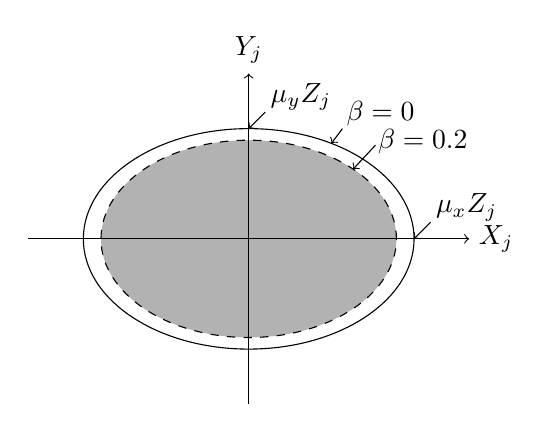
\begin{tikzpicture}[scale = .7]
	% Parameters
	\def\outerX{3}   % x radius of outer ellipse
	\def\outerY{2}   % y radius of outer ellipse
	\def\gap{0.2}    % distance between outer and inner ellipse
	\def\innerX{2.68}
	\def\innerY{1.79}
	
	% Draw outer ellipse
	\draw[] (0,0) ellipse [x radius=\outerX, y radius=\outerY];
	
	% Draw inner ellipse filled with color
	\fill[black!30] (0,0) ellipse [
	x radius={\innerX},
	y radius={\innerY}
	];
	\draw[dashed] (0,0) ellipse [
	x radius={\innerX},
	y radius={\innerY}
	];
	
	% Draw axes
	\draw[->] (-\outerX-1,0) -- (\outerX+1,0) node[right] {$X_j$};
	\draw[->] (0,-\outerY-1) -- (0,\outerY+1) node[above] {$Y_j$};
	
	% Arrows pointing to the ellipses
	\draw[->,thin] (1.7,2) -- ({\outerX*cos(60)},{\outerY*sin(60)}) node[midway, above right] {$\beta=0$};
	\draw[->,thin] (2.3,1.7) -- ({(\innerX)*cos(45)},{(\innerY)*sin(45)}) node[midway, right, shift={(0.05,.2)}] {$\beta=\gap$};
	
	% Arrows pointing to the ellipses
	\draw[->,thin] ({\outerX+.3},.3) -- (\outerX,0) node[midway, above right,shift={(.05,0)}] {$\mu_x Z_j$};
	\draw[->,thin] (.3,{\outerY+.3}) -- (0,\outerY) node[midway, above right,shift={(.05,0)}] {$\mu_y Z_j$};
	
\end{tikzpicture}}
	\hfill
	\adjustbox{valign=c}{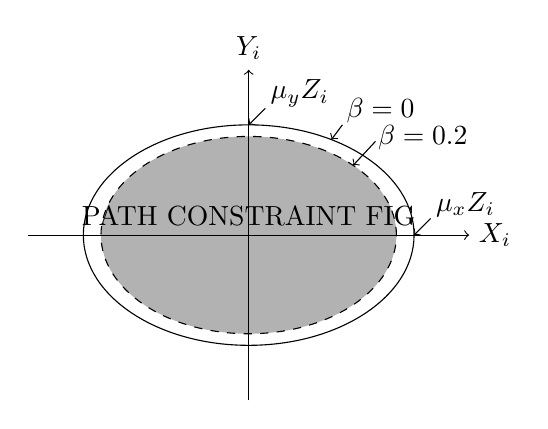
\begin{tikzpicture}[scale = .7]
	% Parameters
	\def\outerX{3}   % x radius of outer ellipse
	\def\outerY{2}   % y radius of outer ellipse
	\def\gap{0.2}    % distance between outer and inner ellipse
	\def\innerX{2.68}
	\def\innerY{1.79}
	
	% Draw outer ellipse
	\draw[] (0,0) ellipse [x radius=\outerX, y radius=\outerY];
	
	% Draw inner ellipse filled with color
	\fill[black!30] (0,0) ellipse [
	x radius={\innerX},
	y radius={\innerY}
	];
	\node[above] at (0,0) {PATH CONSTRAINT FIG};
	\draw[dashed] (0,0) ellipse [
	x radius={\innerX},
	y radius={\innerY}
	];
	
	% Draw axes
	\draw[->] (-\outerX-1,0) -- (\outerX+1,0) node[right] {$X_i$};
	\draw[->] (0,-\outerY-1) -- (0,\outerY+1) node[above] {$Y_i$};
	
	% Arrows pointing to the ellipses
	\draw[->,thin] (1.7,2) -- ({\outerX*cos(60)},{\outerY*sin(60)}) node[midway, above right] {$\beta=0$};
	\draw[->,thin] (2.3,1.7) -- ({(\innerX)*cos(45)},{(\innerY)*sin(45)}) node[midway, right, shift={(0.05,.2)}] {$\beta=\gap$};
	
	% Arrows pointing to the ellipses
	\draw[->,thin] ({\outerX+.3},.3) -- (\outerX,0) node[midway, above right,shift={(.05,0)}] {$\mu_x Z_i$};
	\draw[->,thin] (.3,{\outerY+.3}) -- (0,\outerY) node[midway, above right,shift={(.05,0)}] {$\mu_y Z_i$};
	
\end{tikzpicture}}
	\caption{Graphical representation of the two constraints analyzed in this section: the friction limit constraint in the $X_jY_j$ plane (left panel), and the track limit constraint in the $xy$ plane (right panel). In both figures, the filled gray area bounded by a dashed line indicates the accessible region in the presence of a back-off term.
	}
		%Graphical representation of the two constraints analyzed in the section. The left panel shows the friction limit constraint in the plane $X_j-Y_j$. The ellipse in solid line, whose semi-axes are given by $\mu_{x,j}Z_j$ and $\mu_{y,j}Z_j$, represents the border of the available region for the base constraint, without back-off. The ellipse in dashed line delimits the available region when a back-off $\be^\textrm{FLC}_j=0.2$ is present. This ellipse has its semi-axes reduced by a factor $\sqrt{1-\be^\textrm{FLC}_j}$ w.r.t. the one in solid line.}
	\label{fig:robust_constraints}
\end{figure}

\subsection{Robust track limit constraint formulation}
\label{sec:TLC}
An track limit constraint is required to ensure that the vehicle remains within the circuit boundaries. The formulation adopted introduces an algebraic variable $e$, which satisfies the following constraint:
\begin{equation}
	\begin{Bmatrix}
		x\\y
	\end{Bmatrix}
	-\boldsymbol{c} - e\bn=\boldsymbol{0} \label{eq:onplane_constraint}
\end{equation}
%\begin{equation}
%	\bp-\boldsymbol{c}_k - e_k\bn_k=\boldsymbol{0} \label{eq:onplane_constraint}
%\end{equation}
where $\boldsymbol{c}$ indicates the position of the centerline, and $\bn$ is the unit normal vector to the centerline. Equation~\eqref{eq:onplane_constraint} constraints the CoM of the vehicle to lie on the vertical plane defined by the unit normal vector $\bn$. The previously introduced algebraic variable $e$ is further constrained to take values between $e_\textrm{min}$ and $e_\textrm{max}$, which are determined based on the width of the circuit and the vehicle's front and rear tracks.

In order to take into account for the back-off terms, the maximum and minimum values are modified coherently, so that:
\begin{equation}
	e_\textrm{min} + \be^\textrm{TLC} \leq e \leq e_\textrm{max} - \be^\textrm{TLC}\label{eq:TLC}
\end{equation}
where $\be^\textrm{TLC}$ is computed by considering that the gradient of the constraint w.r.t. the state vector $\na_{\bx}h^\textrm{TLC}$ depends solely on $\bn$.
%Adding a back-off to this constraint produces the same effect as an increase of the front and rear tracks of the vehicle does. 